\section{Ejemplo 6}

    \lipsum[1]
    
    \begin{figure}[h]
    	\centering
    	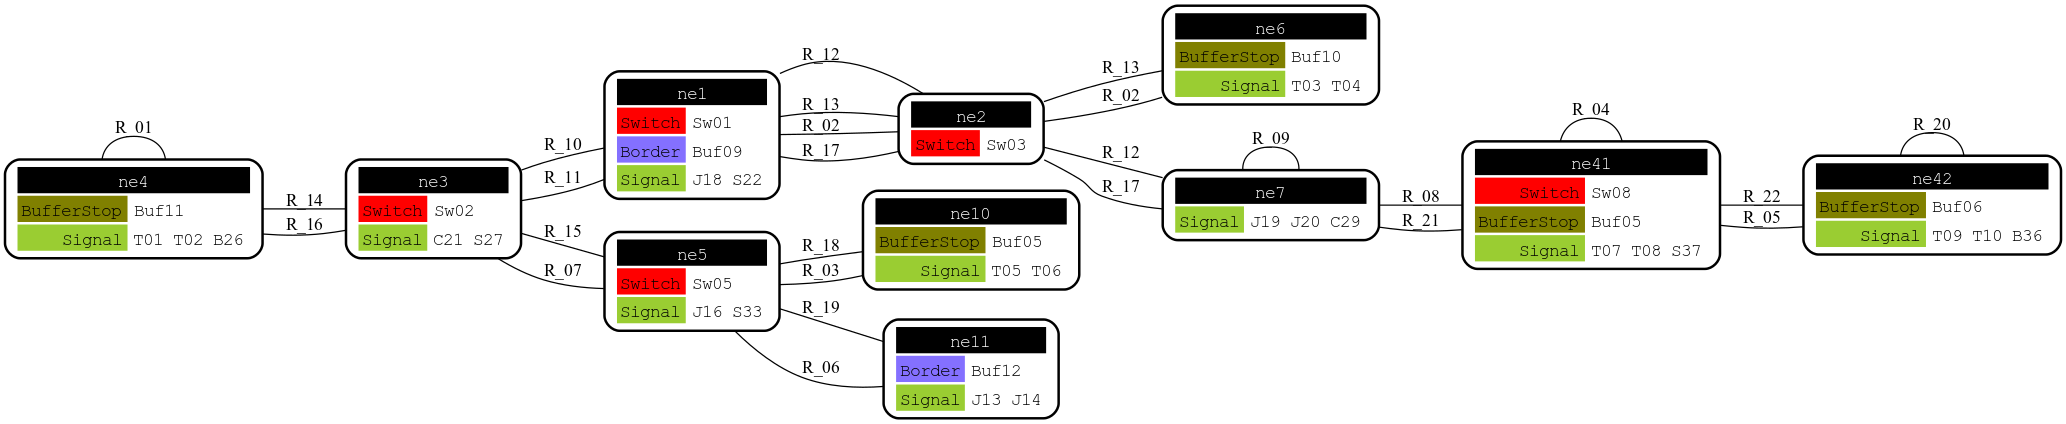
\includegraphics[width=1\textwidth]{Figuras/Graph_6}
    	\centering\caption{XXXX}
    	%\label{fig:LC_P2}
    \end{figure}
    
    \lipsum[1]

    \begin{figure}[h]
        \centering
        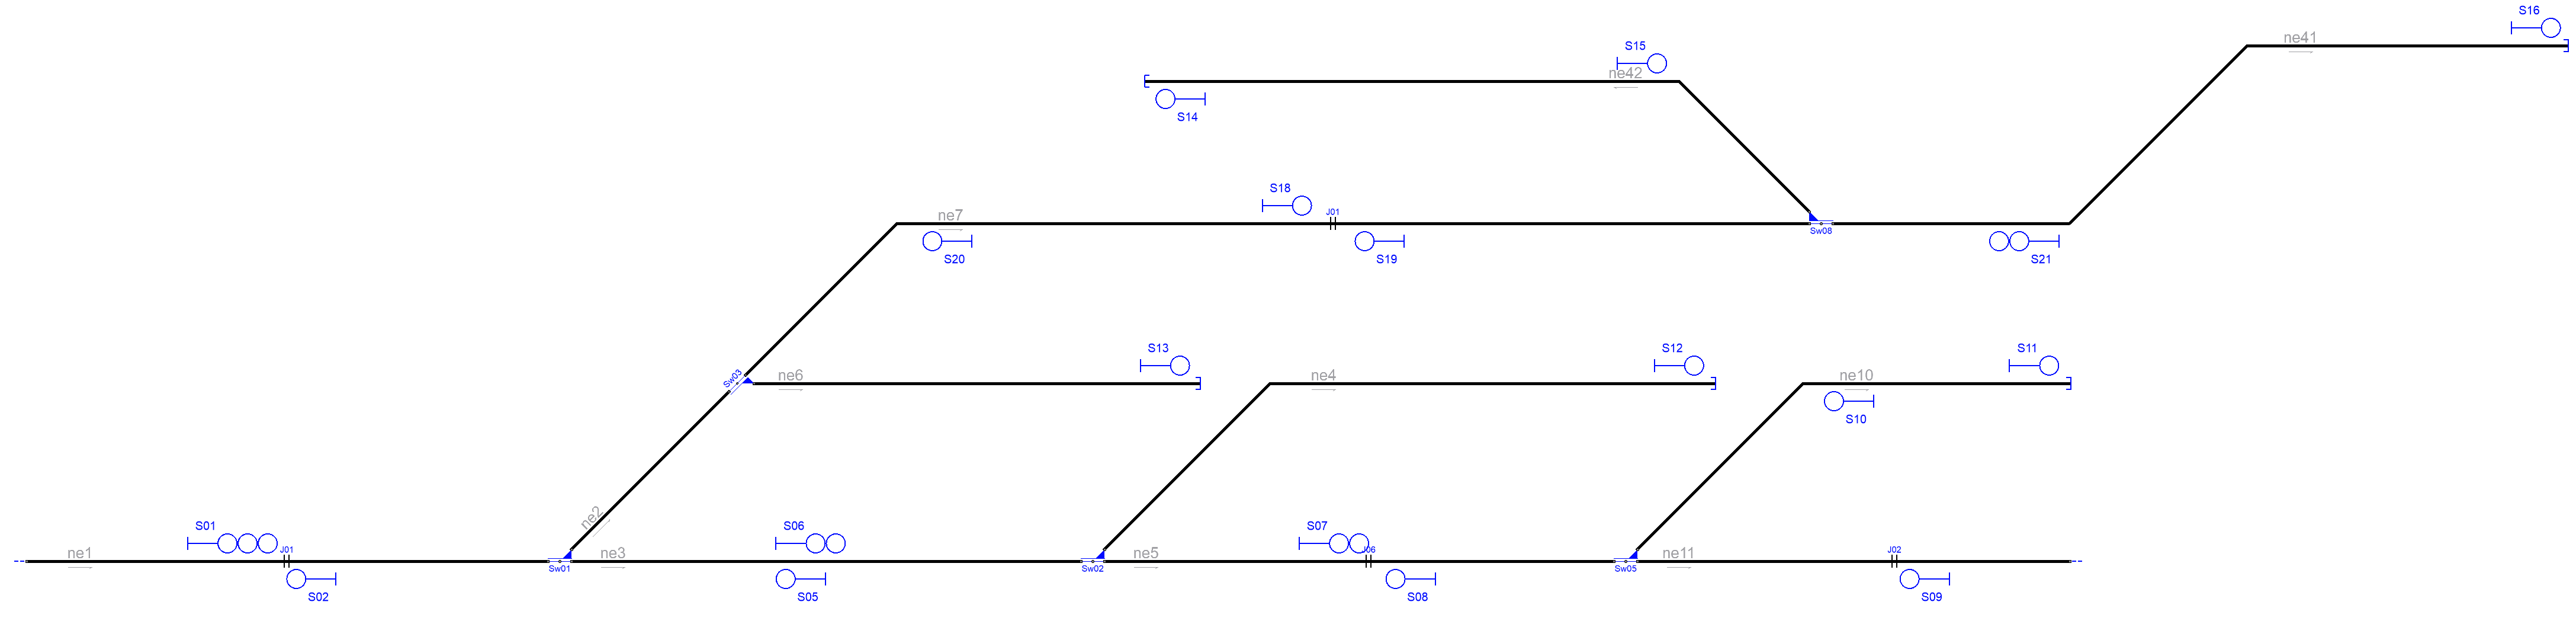
\includegraphics[width=1\textwidth]{resultados-obtenidos/ejemplo6/images/6_original.png}
        \centering\caption{Señalamiento original del ejemplo 6.}
        %\label{fig:LC_P2}
    \end{figure}

    \begin{figure}[h]
        \centering
        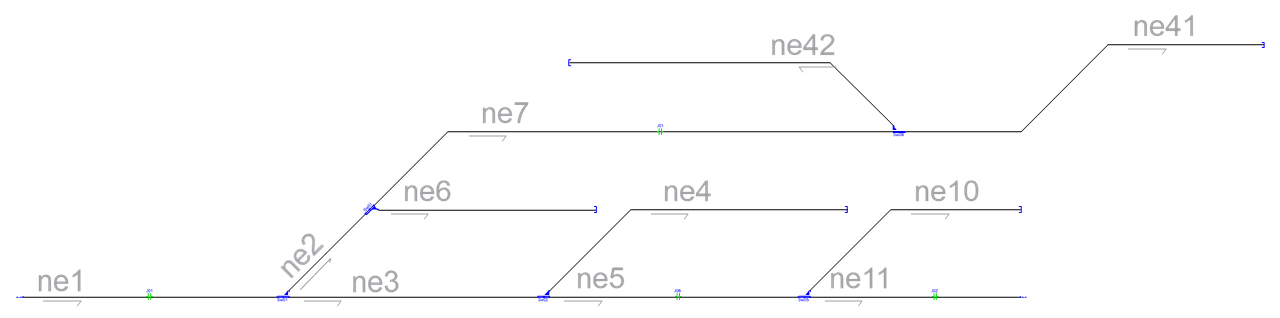
\includegraphics[width=1\textwidth]{resultados-obtenidos/ejemplo6/images/6_empty.png}
        \centering\caption{Topología ferroviaria del ejemplo 6 sin señalamiento.}
        %\label{fig:LC_P2}
    \end{figure}

    \begin{figure}[h]
        \centering
        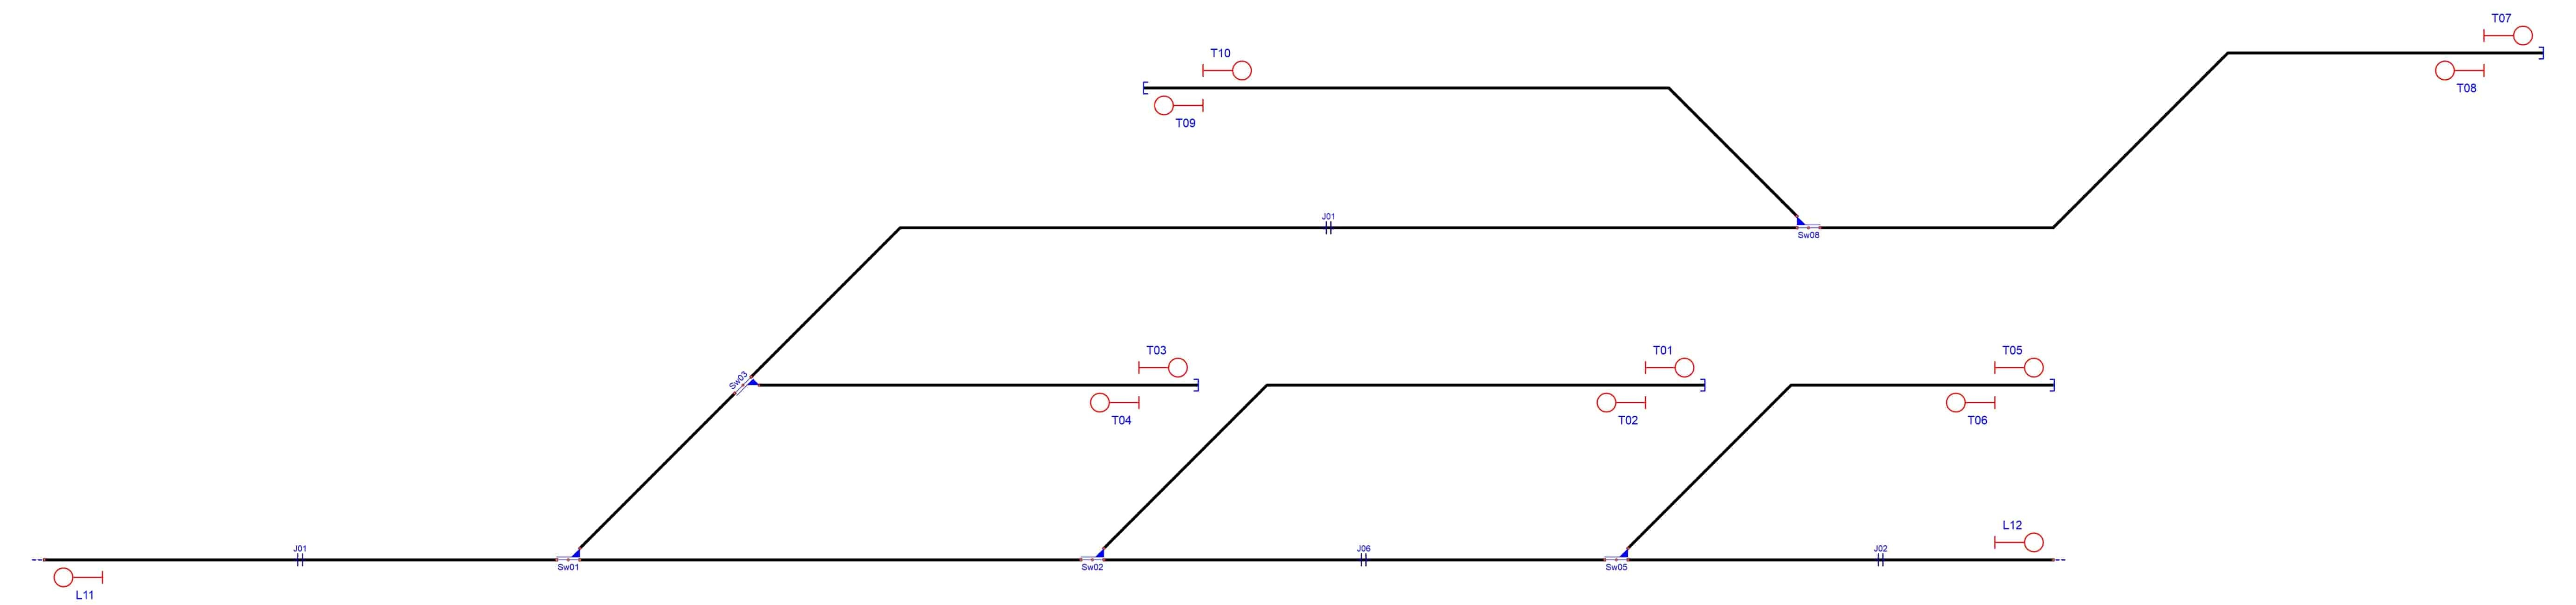
\includegraphics[width=1\textwidth]{resultados-obtenidos/ejemplo6/images/6_step1.png}
        \centering\caption{Señalamiento generado por el RNA para proteger el fín de vía.}
        %\label{fig:LC_P2}
    \end{figure}

    \begin{figure}[h]
        \centering
        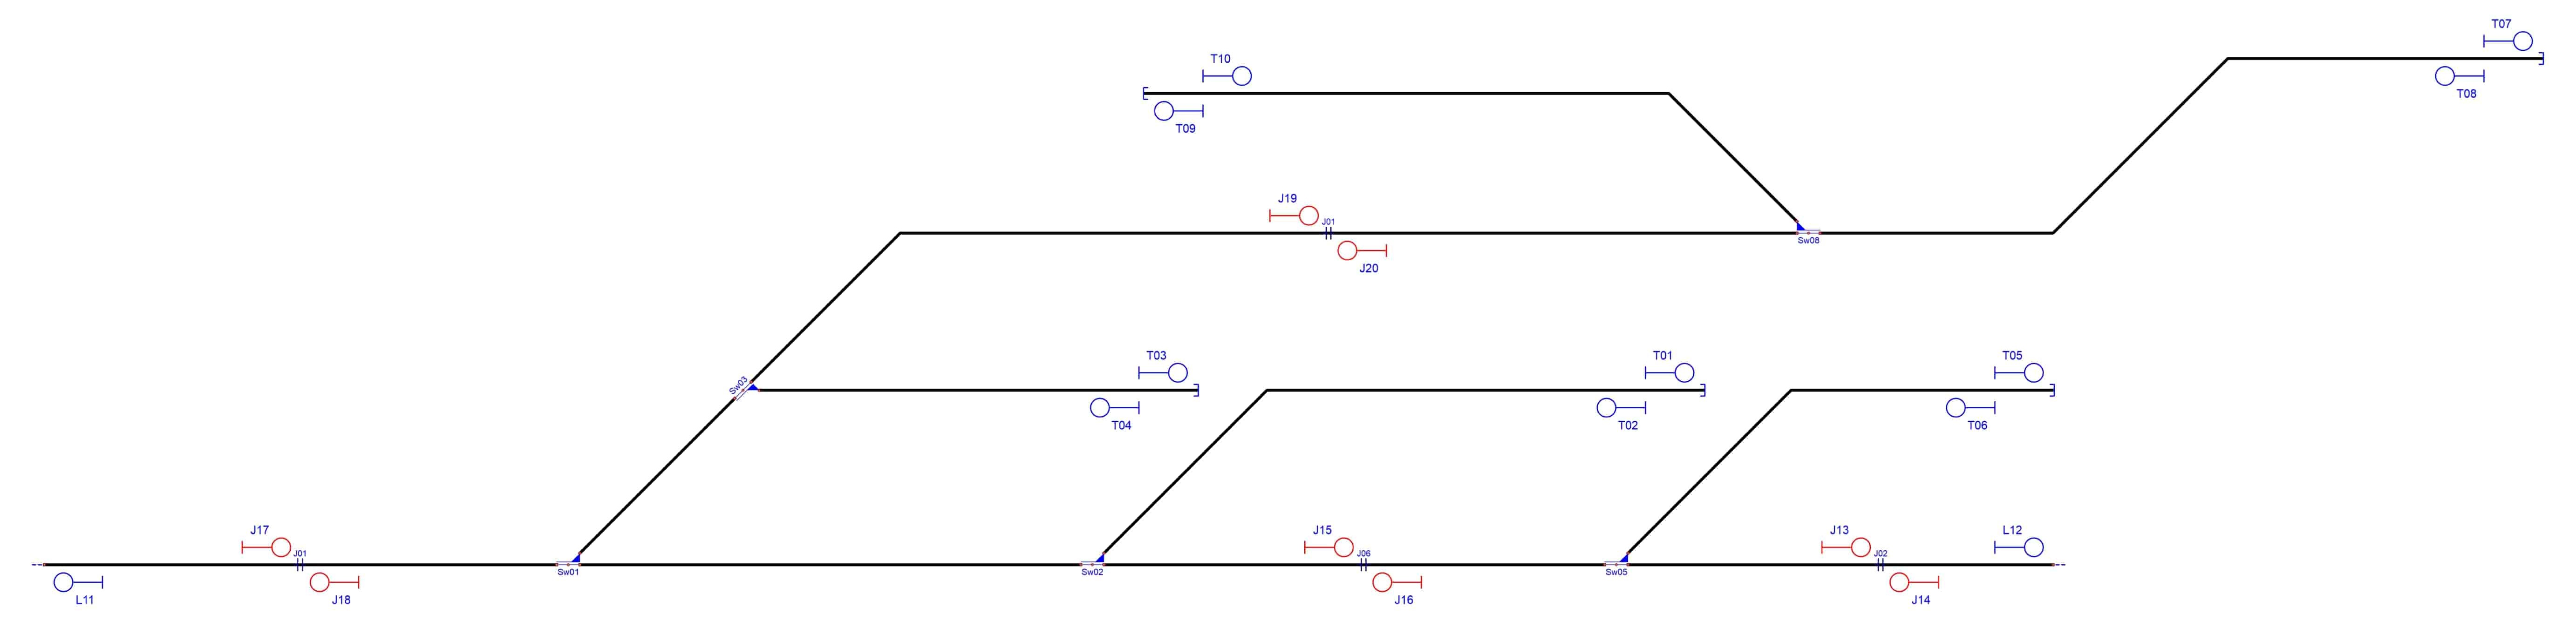
\includegraphics[width=1\textwidth]{resultados-obtenidos/ejemplo6/images/6_step2.png}
        \centering\caption{Señalamiento generado por el RNA para proteger las junturas.}
        %\label{fig:LC_P2}
    \end{figure}

    \begin{figure}[h]
        \centering
        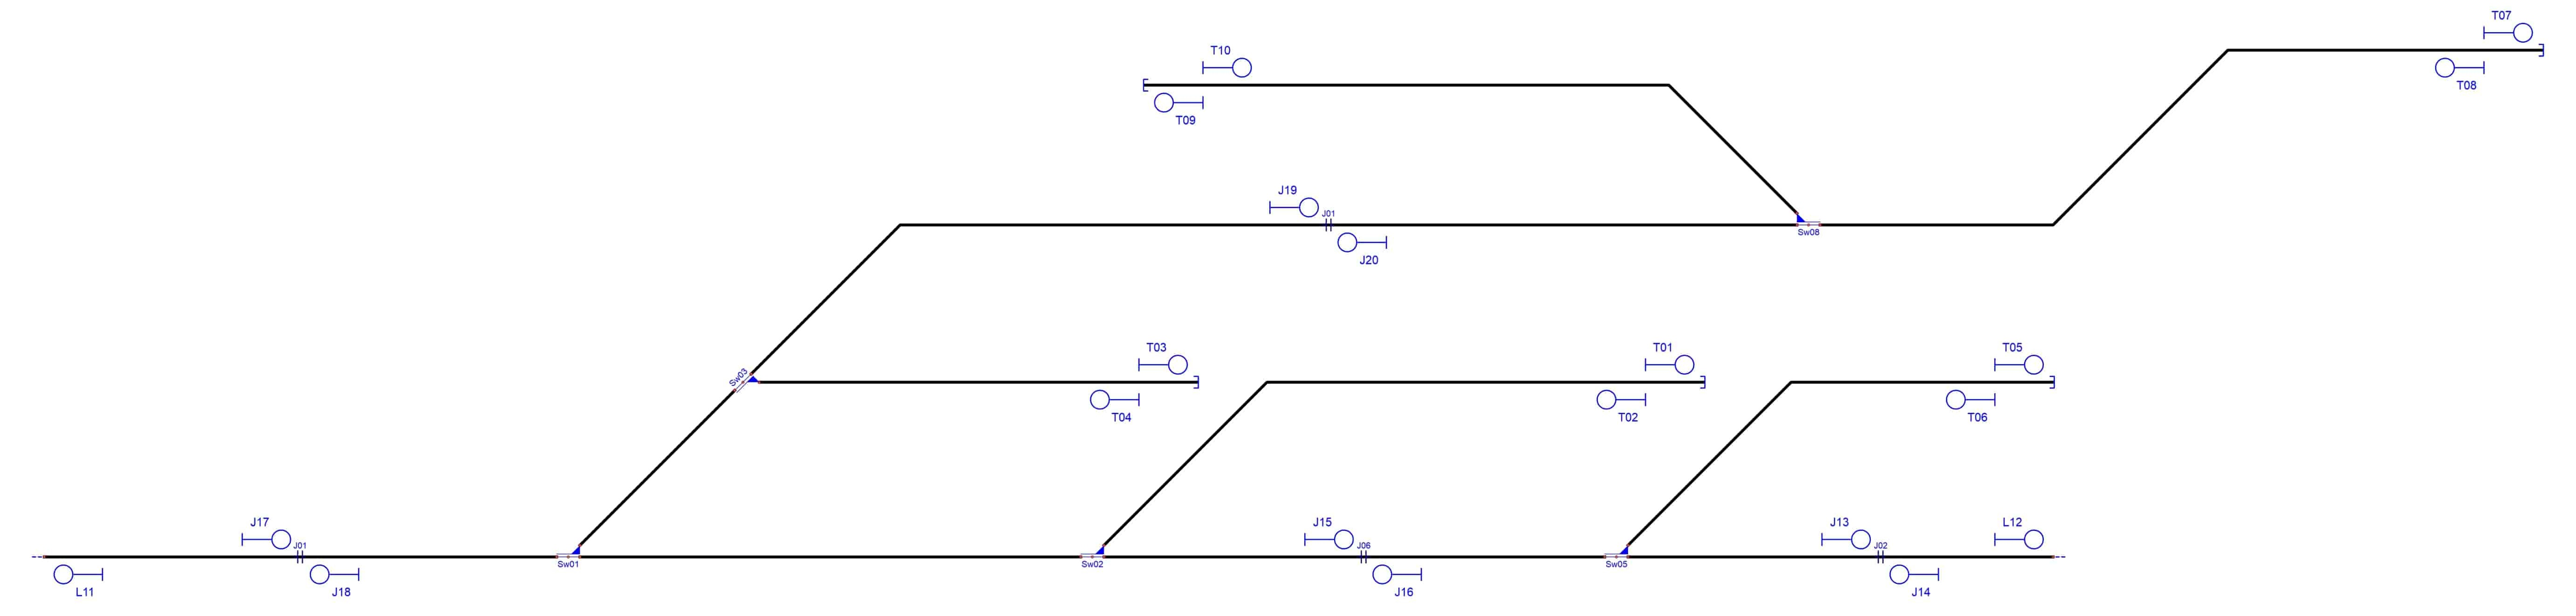
\includegraphics[width=1\textwidth]{resultados-obtenidos/ejemplo6/images/6_step3.png}
        \centering\caption{Señalamiento generado por el RNA para proteger plataformas y cruces de vía.}
        %\label{fig:LC_P2}
    \end{figure}

    \begin{figure}[h]
        \centering
        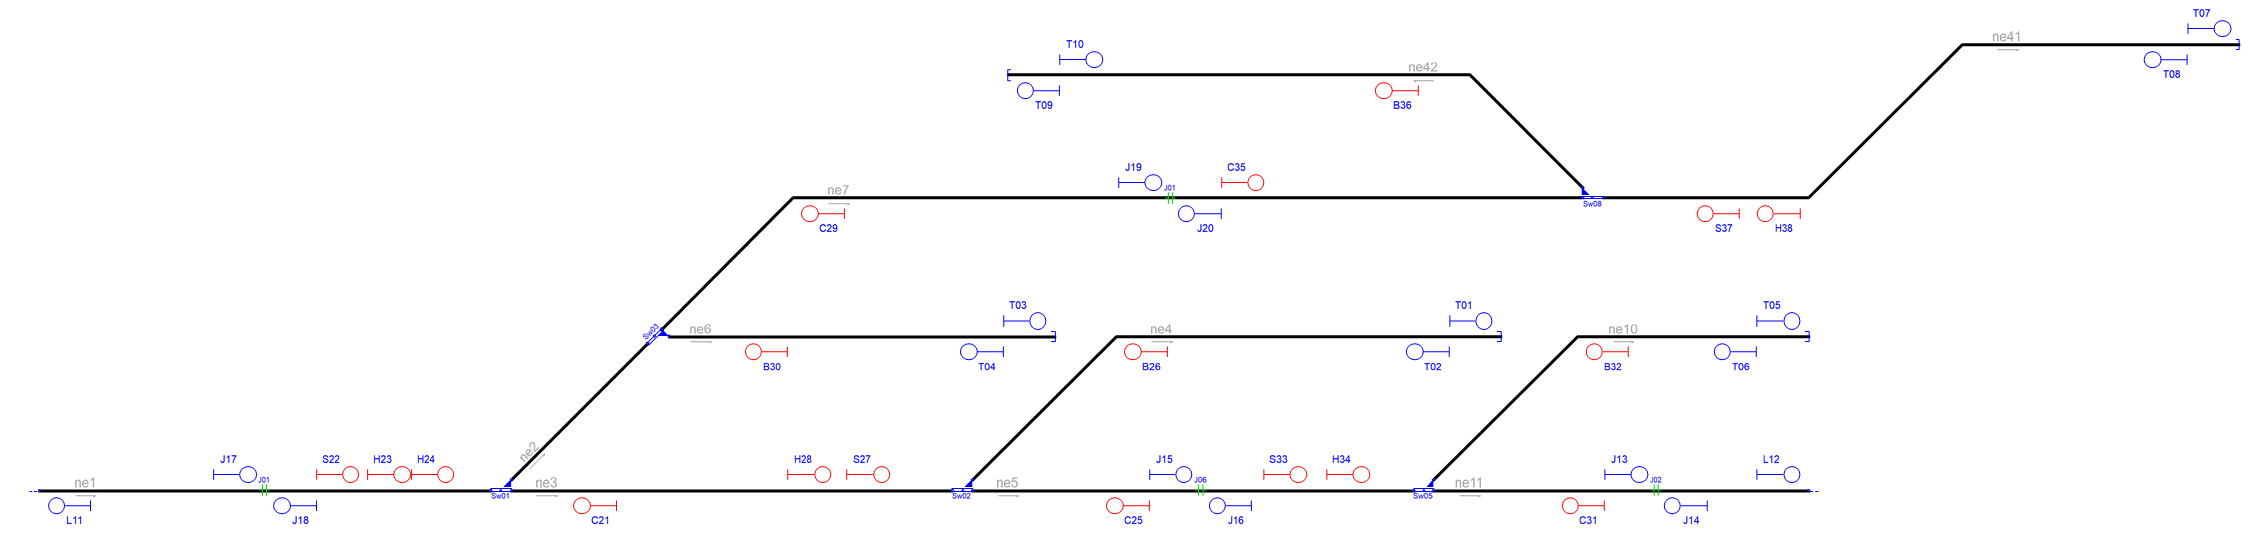
\includegraphics[width=1\textwidth]{resultados-obtenidos/ejemplo6/images/6_step4.png}
        \centering\caption{Señalamiento generado por el RNA para proteger las máquinas de cambios.}
        %\label{fig:LC_P2}
    \end{figure}

    \begin{figure}[h]
        \centering
        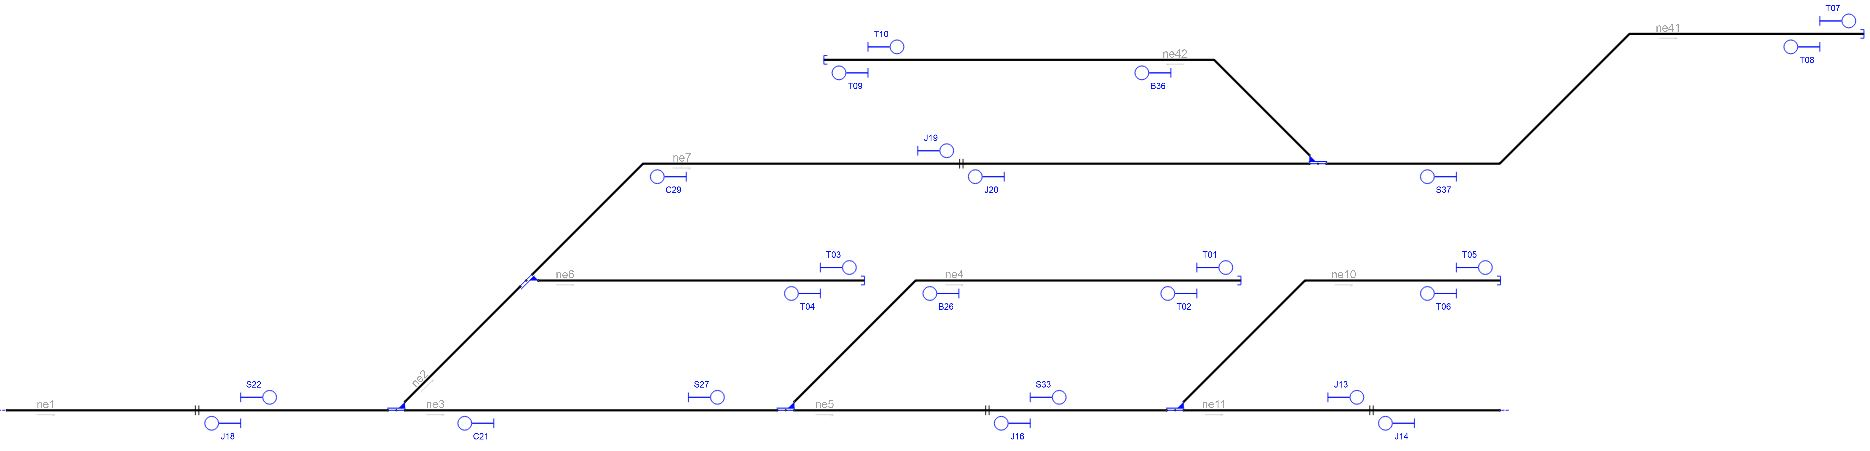
\includegraphics[width=1\textwidth]{resultados-obtenidos/ejemplo6/images/6_RNA.png}
        \centering\caption{Señalamiento generado y simplificado por el RNA.}
        %\label{fig:LC_P2}
    \end{figure}
    
    \section{Señalamiento original}

    El señalamiento original, ilustrado en la Figura \ref{fig:EJ6_2}, incluye señales de parada próximas a los finales de vías absolutos (S11, S12, S13, S14, S16), señales de maniobras antes de converger en una vía principal (S10, S15, S20) y señales múltiples para cambios de vías divergentes (S01, S06, S07, S21), entre varias otras señales.
    
    \begin{figure}[H]
    	\centering
    	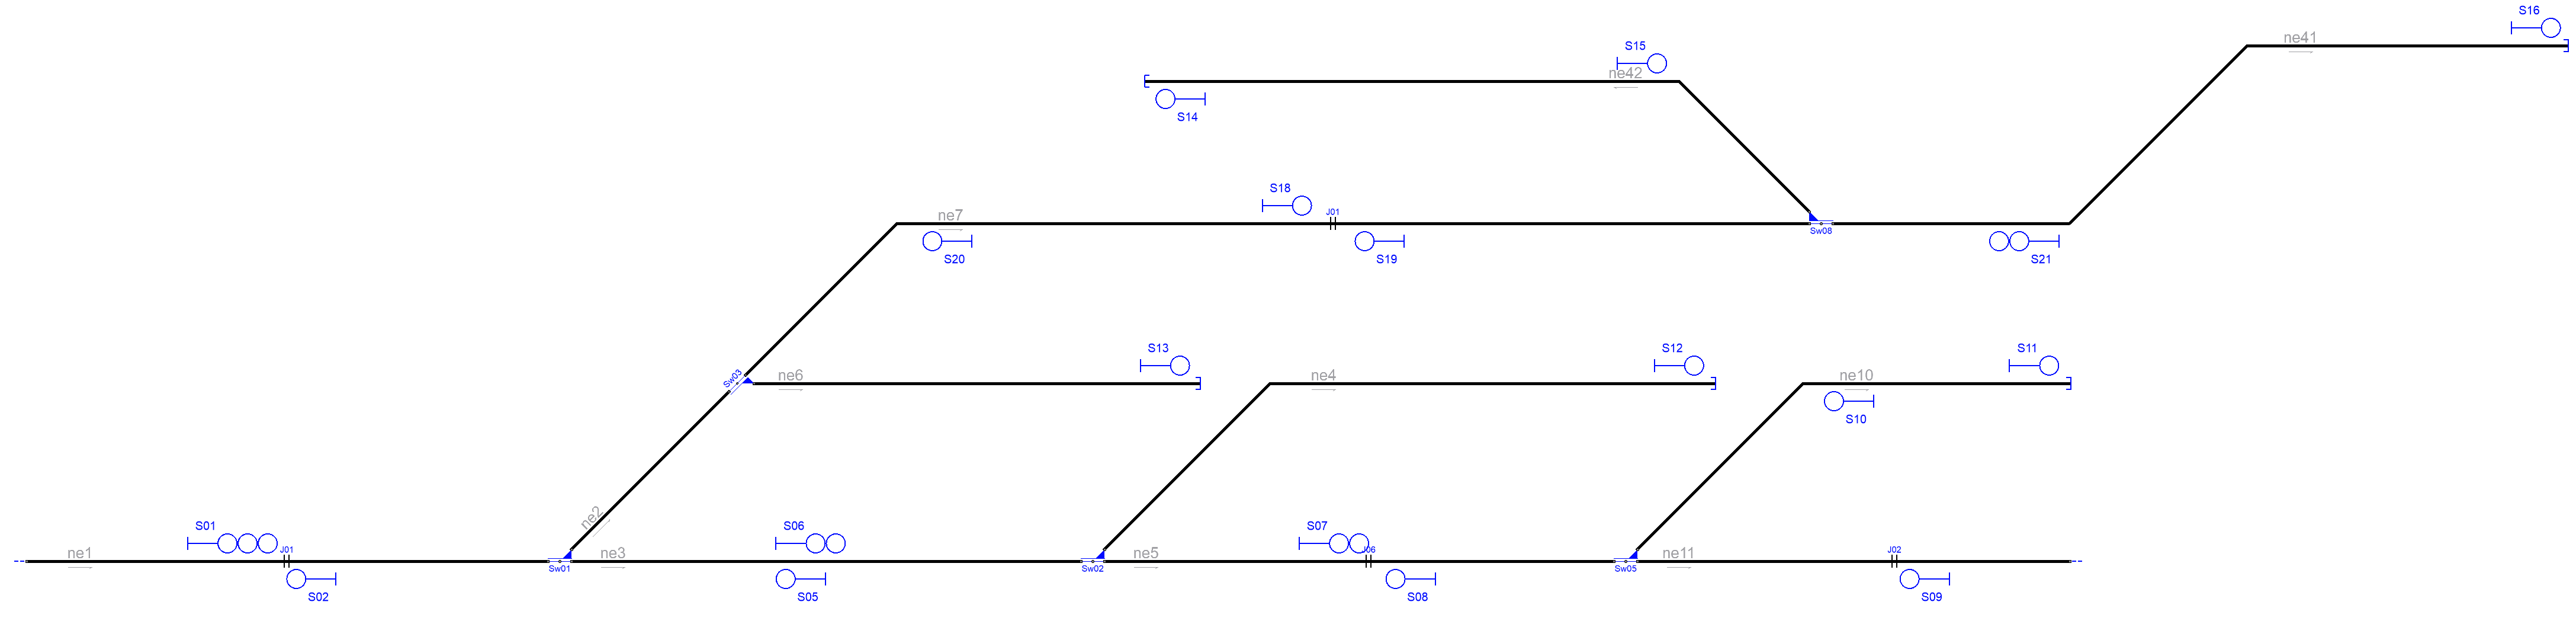
\includegraphics[width=1\textwidth]{resultados-obtenidos/ejemplo6/images/6_original.png}
    	\centering\caption{Señalamiento original del ejemplo 6.}
    	\label{fig:EJ6_2}
    \end{figure}
    
    Estas señales permiten definir hasta un máximo de 16 rutas, todas ellas detalladas en la Tabla \ref{Tab:tabla_original_6}. En una primera inspección, se puede comprobar que todos los elementos ferroviarios son alcanzados por al menos una de las rutas, en al menos una dirección. Además, todos los cambios de vías son utilizados, de forma simple o compuesta. 
    
    \begin{table}[H]
        {
        \caption{Tabla de enclavamiento original del ejemplo 6.}
        \label{Tab:tabla_original_6}
        \centering
        \resizebox{1\textwidth}{!}{
            \begin{tabular}{ c c c c c c c }
                \hline	
                    Ruta & Inicio & Final & Cambio & Plataforma & Cruce & netElement \\	
                \hline
                    R$_{01}$  & S$_{01}$ & S$_{06}$ & Sw$_{01}^{N}$ & - & - & ne$_{01}$-ne$_{03}$\\
                    R$_{02}$  & S$_{01}$ & S$_{13}$ & Sw$_{01}^{R}$+Sw$_{03}^{R}$ & - & - & ne$_{01}$-ne$_{06}$\\
                    R$_{03}$  & S$_{01}$ & S$_{18}$ & Sw$_{01}^{R}$+Sw$_{03}^{R}$ & - & - & ne$_{01}$-ne$_{07}$\\
                    R$_{04}$  & S$_{06}$ & S$_{07}$ & Sw$_{02}^{N}$ & - & - & ne$_{03}$-ne$_{05}$\\
                    R$_{05}$  & S$_{06}$ & S$_{12}$ & Sw$_{02}^{R}$ & - & - & ne$_{03}$-ne$_{04}$\\
                    R$_{06}$  & S$_{21}$ & S$_{19}$ & Sw$_{08}^{N}$ & - & - & ne$_{41}$-ne$_{07}$\\
                    R$_{07}$  & S$_{21}$ & S$_{14}$ & Sw$_{08}^{R}$ & - & - & ne$_{41}$-ne$_{42}$\\
                    R$_{08}$  & S$_{05}$ & S$_{02}$ & Sw$_{01}^{N}$ & - & - & ne$_{03}$-ne$_{01}$\\
                    R$_{09}$  & S$_{09}$ & S$_{08}$ & Sw$_{05}^{N}$ & - & - & ne$_{11}$-ne$_{05}$\\
                    R$_{10}$  & S$_{08}$ & S$_{05}$ & Sw$_{02}^{N}$ & - & - & ne$_{05}$-ne$_{03}$\\
                    R$_{11}$  & S$_{10}$ & S$_{08}$ & Sw$_{05}^{R}$ & - & - & ne$_{10}$-ne$_{05}$\\
                    R$_{12}$  & S$_{15}$ & S$_{16}$ & Sw$_{08}^{R}$ & - & - & ne$_{42}$-ne$_{41}$\\
                    R$_{13}$  & S$_{18}$ & S$_{16}$ & Sw$_{08}^{N}$ & - & - & ne$_{07}$-ne$_{41}$\\
                    R$_{14}$  & S$_{19}$ & S$_{20}$ & - & - & - & ne$_{07}$\\
                    R$_{15}$  & S$_{20}$ & S$_{02}$ & Sw$_{01}^{R}$+Sw$_{03}^{N}$ & - & - & ne$_{07}$-ne$_{01}$\\
                    R$_{16}$  & S$_{07}$ & S$_{11}$ & Sw$_{05}^{R}$ & - & - & ne$_{05}$-ne$_{10}$\\
                \hline
            \end{tabular}
        }
     }
    \end{table}
    
    Algunas rutas abarcan mas de un \textit{netElement}, como por ejemplo la ruta R15 que comienza en la señal S20 y finaliza en la señal S02, atravesando los \textit{netElements} ne07 y ne01, utilizando los cambios de vías Sw01 y Sw03, en posición reversa y normal respectivamente.
    \section{Señalamiento generado por el RNA}

    El RNA también exporta la información mostrada en el Código \ref{lst:EJ6_8} en una hoja de cálculo, similar a la que se visualiza en la Tabla \ref{Tab:tabla_generated_6}.
    
    \begin{table}[H]
        {
        \caption{Tabla de enclavamiento del ejemplo 6 generada por el RNA.}
        \label{Tab:tabla_generated_6}
        %\centering
        \begin{center}      
        	\resizebox{0.8\textwidth}{!}{
            \begin{tabular}{ c c c c c c c }
                \hline	
                    Ruta & Inicio & Final & Cambio & Plataforma & Cruce & netElement \\	
                \hline
                    R$_{01}$  & T$_{02}$ & B$_{26}$ & - & - & - & ne$_{04}$\\
                    R$_{02}$  & T$_{04}$ & J$_{18}$ & Sw$_{01}^{R}$+Sw$_{03}^{R}$ & - & - & ne$_{06}$-ne$_{01}$\\
                    R$_{03}$  & T$_{06}$ & J$_{16}$ & Sw$_{05}^{R}$ & - & - & ne$_{10}$-ne$_{05}$\\
                    R$_{04}$  & T$_{08}$ & S$_{37}$ & - & - & - & ne$_{41}$\\
                    R$_{05}$  & T$_{10}$ & T$_{07}$ & Sw$_{08}^{R}$ & - & - & ne$_{42}$-ne$_{41}$\\
                    R$_{06}$  & J$_{14}$ & J$_{16}$ & Sw$_{05}^{N}$ & - & - & ne$_{11}$-ne$_{05}$\\
                    R$_{07}$  & J$_{16}$ & C$_{21}$ & Sw$_{02}^{N}$ & - & - & ne$_{05}$-ne$_{03}$\\
                    R$_{08}$  & J$_{19}$ & T$_{07}$ & Sw$_{08}^{N}$ & - & - & ne$_{07}$-ne$_{41}$\\
                    R$_{09}$  & J$_{20}$ & C$_{29}$ & - & - & - & ne$_{07}$\\
                    R$_{10}$  & C$_{21}$ & J$_{18}$ & Sw$_{01}^{N}$ & - & - & ne$_{03}$-ne$_{01}$\\
                    R$_{11}$  & S$_{22}$ & S$_{27}$ & Sw$_{01}^{N}$ & - & - & ne$_{01}$-ne$_{03}$\\
                    R$_{12}$  & S$_{22}$ & J$_{19}$ & Sw$_{01}^{R}$+Sw$_{03}^{N}$ & - & - & ne$_{01}$-ne$_{07}$\\
                    R$_{13}$  & S$_{22}$ & T$_{03}$ & Sw$_{01}^{R}$+Sw$_{03}^{R}$ & - & - & ne$_{01}$-ne$_{06}$\\
                    R$_{14}$  & B$_{26}$ & C$_{21}$ & Sw$_{02}^{R}$ & - & - & ne$_{04}$-ne$_{03}$\\
                    R$_{15}$  & S$_{27}$ & S$_{33}$ & Sw$_{02}^{N}$ & - & - & ne$_{03}$-ne$_{05}$\\
                    R$_{16}$  & S$_{27}$ & T$_{01}$ & Sw$_{02}^{R}$ & - & - & ne$_{03}$-ne$_{04}$\\
                    R$_{17}$  & C$_{29}$ & J$_{18}$ & Sw$_{01}^{R}$+Sw$_{03}^{N}$ & - & - & ne$_{07}$-ne$_{01}$\\
                    R$_{18}$  & S$_{33}$ & J$_{13}$ & Sw$_{05}^{N}$ & - & - & ne$_{05}$-ne$_{11}$\\
                    R$_{19}$  & S$_{33}$ & T$_{05}$ & Sw$_{05}^{R}$ & - & - & ne$_{05}$-ne$_{10}$\\
                    R$_{20}$  & B$_{36}$ & T$_{09}$ & - & - & - & ne$_{42}$\\
                    R$_{21}$  & S$_{37}$ & J$_{20}$ & Sw$_{08}^{N}$ & - & - & ne$_{41}$-ne$_{07}$\\
                    R$_{22}$  & S$_{37}$ & B$_{36}$ & Sw$_{08}^{R}$ & - & - & ne$_{41}$-ne$_{42}$\\
                \hline
            \end{tabular}
        }
        \end{center}
     }
    \end{table}
    
    En una primera inspección podemos ver que el nuevo señalamiento tiene 22 rutas, versus las 16 rutas del señalamiento original (ver Tabla \ref{Tab:tabla_original_6}). Esto se debe a que todas las vías son consideradas de ambos sentidos por el RNA, lo cuál queda de manifiesto cuando se comprueba que todas las plataformas y cruces de vía son atravesados por dos rutas, una en cada dirección. 
    \section{Sistema generado por el ACG}
	
	En base a la red de grafos, ilustrada en la Figura \ref{fig:EJ6_8}, el ACG determinó la siguiente cantidad de elementos, tal puede visualizarse en el Código \ref{lst:EJ6_8}.
	
	\begin{lstlisting}[language = {}, caption = Cantidad de elementos a implementar por el ACG, label = {lst:EJ6_8}]
	n_netElements:11
	n_switch:5
	n_doubleSwitch:0
	n_borders:2
	n_buffers:5
	n_levelCrossings:0
	n_platforms:0
	n_scissorCrossings:0
	n_signals:24
	N : 62
	\end{lstlisting}
	
	Se repetirán los pasos detallados en el ejemplo 1, Sección \ref{sec:EJEMPLO1_ACG}, por lo que solamente se destacarán aspectos particulares de este ejemplo. El ACG genera 80 archivos en formato VHDL. El archivo \textit{Arty\_Z7-10.XDC} es el mismo para todos los ejemplos, al ser invariante respecto a la cantidad de pines a utilizar. Se deberá modificar el script mostrado en el Código \ref{lst:EJ1_script} y cambiar el parámetro \textit{chosen} a 6 para automatizar la importación de los archivos del ejemplo 6 y desvincular cualquier otro conjunto de archivos de ejemplos anteriores.
	
	Una vez ejecutado el script, Vivado ordenará los archivos de forma jerárquica, donde el módulo \textit{global} incluye todos los módulos que fueron detallados en la Sección \ref{sec:interlockingArch}. Cada una de las instancias del módulo \textit{network} contienen sus propias 62 instancias de los mismos módulos de cada elemento ferroviario ya que N, cantidad de elementos ferroviarios, es 62 en el Código \ref{lst:EJ6_8}. El ejemplo 6 utiliza mas de 19870 sub módulos conectados automáticamente mediante mas de 37910 señales, lo cual se aleja bastante de un desarrollo que pueda realizarse manualmente de forma trivial.
	
	Cuando Vivado genera el diagrama de bloques ya tenemos la certeza de que el código VHDL ha pasado la prueba de sintaxis del entorno de desarrollo. A continuación, se deberá sintetizar e implementar el sistema para generar el bitstream que será utilizado para programar la FPGA. Los procesos de síntesis e implementación fueron detallados en el ejemplo 1, Sección \ref{sec:EJEMPLO1_ACG}.
	
	Los resultados de ambos procesos son detallados en la Tabla \ref{Tab:tabla_ACG_6}. Los porcentajes de uso son calculados por Vivado automáticamente, teniendo en cuenta que la plataforma Arty Z7 20 posee 53200 Look-Up-Tables (LUTs), 106400 Flip-Flops (FFs), 125 Pines de entrada y salida (IOs) y 32 Buffers (BUFGs), tal cómo se explicó en la Sección \ref{sec:AGG}. En este ejemplo, la cantidad de recursos utilizados es baja y el tiempo de síntesis e implementación es de 49 y 1 minuto con 10 segundos, respectivamente.
	
	\begin{table}[H]
		{
			\caption{Síntesis e implementación del ejemplo 6 generado por el ACG.}
			\label{Tab:tabla_ACG_6}
			\centering
			%\small
			%\centering
			\begin{center}
				\resizebox{0.7\textwidth}{!}{
					\begin{tabular}{ c c c c }
						\hline	
						Recursos & Síntesis & Implementación & Uso \\	
						\hline
						LUT & 3388 & 3348 & 6.37-6.29\%\\
						FF & 3793 & 3796 & 3.56-3.57\%\\
						IO & 15 & 15 & 12.00\%\\
						BUFG & 3 & 3 & 9.38\%\\
						\hline
					\end{tabular}
				}
			\end{center}
		}    
	\end{table}
    \subsection{Validacion del sistema}

    \lipsum[1]

    \begin{table}[!h]
        {
        \caption{Equivalencias entre las rutas originales y las generadas por el RNA.}
        \label{Tab:tabla_validation_6}
        \centering
        %\small
            %\centering
            \begin{center}
            \resizebox{1\textwidth}{!}{
            \begin{tabular}{ c c c c }
                \hline	
                    Original & Señales & RNA & Señales \\	
                \hline
                    R$_{01}$ & S$_{01}$-S$_{06}$ & R$_{11}$ & S$_{22}$-S$_{27}$ \\
                    R$_{02}$ & S$_{01}$-S$_{13}$ & R$_{13}$ & S$_{22}$-T$_{03}$ \\
                    R$_{03}$ & S$_{01}$-S$_{18}$ & R$_{12}$ & S$_{22}$-J$_{19}$ \\
                    R$_{04}$ & S$_{06}$-S$_{07}$ & R$_{15}$ & S$_{27}$-S$_{33}$ \\
                    R$_{05}$ & S$_{06}$-S$_{12}$ & R$_{16}$ & S$_{27}$-T$_{01}$ \\
                    R$_{06}$ & S$_{21}$-S$_{19}$ & R$_{21}$ & S$_{37}$-J$_{20}$ \\
                    R$_{07}$ & S$_{21}$-S$_{14}$ & R$_{22}$ & S$_{37}$-B$_{36}$ \\
                    R$_{08}$ & S$_{05}$-S$_{02}$ & R$_{10}$ & C$_{21}$-J$_{18}$ \\
                    R$_{09}$ & S$_{09}$-S$_{08}$ & R$_{06}$ & J$_{14}$-J$_{16}$ \\
                    R$_{10}$ & S$_{08}$-S$_{05}$ & R$_{07}$ & J$_{16}$-C$_{21}$ \\
                    R$_{11}$ & S$_{10}$-S$_{08}$ & R$_{03}$ & T$_{06}$-J$_{16}$ \\
                    R$_{12}$ & S$_{15}$-S$_{16}$ & R$_{05}$ & T$_{10}$-T$_{07}$ \\
                    R$_{13}$ & S$_{18}$-S$_{16}$ & R$_{08}$ & J$_{19}$-T$_{07}$ \\
                    R$_{14}$ & S$_{19}$-S$_{20}$ & R$_{08}$ & J$_{20}$-C$_{29}$ \\
                    R$_{15}$ & S$_{20}$-S$_{02}$ & R$_{17}$ & C$_{29}$-J$_{18}$ \\
                    R$_{16}$ & S$_{07}$-S$_{11}$ & R$_{19}$ & S$_{33}$-T$_{05}$ \\
                \hline
            \end{tabular}
            }
            \end{center}
        }    
    \end{table}